\documentclass[10pt]{article}
\usepackage[UTF8]{ctex}

\usepackage[utf8]{inputenc} % allow utf-8 input
\usepackage{url}
\usepackage{bm}
\usepackage{amsmath,amscd}
\usepackage{amssymb,array}
\usepackage{amsfonts,latexsym}
\usepackage{graphicx,subfig,wrapfig}
\usepackage{times}
\usepackage{psfrag,epsfig}
\usepackage{verbatim}
\usepackage{tabularx}
\usepackage[pagebackref=true,breaklinks=true,letterpaper=true,colorlinks,bookmarks=false]{hyperref}
\usepackage{cite}
\usepackage{algorithm}
\usepackage{multirow}
\usepackage{caption}
\usepackage{algorithmic}
\usepackage[amsmath,thmmarks]{ntheorem}
\usepackage{listings}
\usepackage{color}


\newtheorem{thm}{Theorem}
\newtheorem{mydef}{Definition}

\DeclareMathOperator*{\rank}{rank}
\DeclareMathOperator*{\trace}{trace}
\DeclareMathOperator*{\acos}{acos}
\DeclareMathOperator*{\argmax}{argmax}


\renewcommand{\algorithmicrequire}{ \textbf{Input:}}     
\renewcommand{\algorithmicensure}{ \textbf{Output:}}
\renewcommand{\mathbf}{\boldsymbol}
\newcommand{\mb}{\mathbf}
\newcommand{\matlab}[1]{\texttt{#1}}
\newcommand{\setname}[1]{\textsl{#1}}
\newcommand{\Ce}{\mathbb{C}}
\newcommand{\Ee}{\mathbb{E}}
\newcommand{\Ne}{\mathbb{N}}
\newcommand{\Se}{\mathbb{S}}
\newcommand{\norm}[2]{\left\| #1 \right\|_{#2}}

\newenvironment{mfunction}[1]{
	\noindent
	\tabularx{\linewidth}{>{\ttfamily}rX}
	\hline
	\multicolumn{2}{l}{\textbf{Function \matlab{#1}}}\\
	\hline
}{\\\endtabularx}

\newcommand{\parameters}{\multicolumn{2}{l}{\textbf{Parameters}}\\}

\newcommand{\fdescription}[1]{\multicolumn{2}{p{0.96\linewidth}}{
		
		\textbf{Description}
		
		#1}\\\hline}

\newcommand{\retvalues}{\multicolumn{2}{l}{\textbf{Returned values}}\\}
\def\0{\boldsymbol{0}}
\def\b{\boldsymbol{b}}
\def\bmu{\boldsymbol{\mu}}
\def\e{\boldsymbol{e}}
\def\u{\boldsymbol{u}}
\def\x{\boldsymbol{x}}
\def\v{\boldsymbol{v}}
\def\w{\boldsymbol{w}}
\def\N{\boldsymbol{N}}
\def\X{\boldsymbol{X}}
\def\Y{\boldsymbol{Y}}
\def\A{\boldsymbol{A}}
\def\B{\boldsymbol{B}}
\def\y{\boldsymbol{y}}
\def\cX{\mathcal{X}}
\def\transpose{\top} % Vector and Matrix Transpose

%\long\def\answer#1{{\bf ANSWER:} #1}
\long\def\answer#1{}
\newcommand{\myhat}{\widehat}
\long\def\comment#1{}
\newcommand{\eg}{{e.g.,~}}
\newcommand{\ea}{{et al.~}}
\newcommand{\ie}{{i.e.,~}}

\newcommand{\db}{{\boldsymbol{d}}}
\renewcommand{\Re}{{\mathbb{R}}}
\newcommand{\Pe}{{\mathbb{P}}}

\hyphenation{MATLAB}

\usepackage[margin=1in]{geometry}

\begin{document}
	
\title{	Numerical Optimization, 2020 Fall\\Homework 5}
\date{Due on 14:59 OCT 27, 2020\\
	请尽量使用提供的tex模板,单纯形法的表格可手绘拍照加入文档.
	}
\maketitle

%%%%%--------------------
\section*{Production Planning by a Computer Manufacturer}
{\color{red}(建议阅读Bertsimas教材``Introduction to Linear Optimization"的1.2节和5.1节对应内容)}
\subsection*{线性规划建模和求解}
公司Digital Equipment Corperation (DEC)可以生产5种不同的产品(GP-1, GP-2, GP-3, WS-1, WS-2)。五种产品的生产分别需要两种原件(disk drives和256K boards)的数量, 以及五种产品的售价如下表:
\begin{figure}[H]
	\centering
	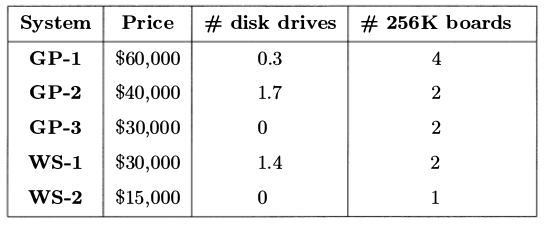
\includegraphics[width=0.55\linewidth]{HW5_1.png}
	%\caption{Accuracy demo.}
	\label{fig.prob1}
\end{figure}
\noindent
在实际生产加工中还有以下约束:
\begin{enumerate}
	\item 五种产品的生产总数不超过7000;
	\item disk drives原材料的供应量在3000个到7000个之间;
	\item 256K boards原材料的供应量在8000个到16000个之间;
	\item GP-1的最大需求不超过1800个, GP-3最大需求不超过300个, GP-1,2,3的总需求不超过3800个, WS-1,2的最大总需求不超过3200个; GP-2的最小需求不低于500个, WS-1的最小需求不低于500个, WS-2的最小需求不低于400个。
\end{enumerate}
由于原材料disk drives和256K boards的总供给量限制, DEC公司给出了对应的解决方案:
\begin{itemize}
	\item 对于disk drives的供给不足提出了\emph{constrained mode:} 仅GP-2需要一个disk drive, WS-1需要一个disk drive, 其他产品的生产均不需要disk drive;
	\item 对于256K boards的供给不足提出了\emph{alternative mode:} GP-1的生产可以用2块alternative boards来替换4块256K boards, alternative boards的供给量为4000块。其他产品不能使用alternative boards。
\end{itemize}
因此, 基于\emph{constrained mode}和\emph{alternative mode}, 我们共有四种可选择的生产方案: 
(方案一):{alternative mode} \& {constrained mode}, (方案二):{alternative mode} \& {unconstrained mode}, (方案三): not use {alternative mode} \& {constrained mode}, (方案四):not use {alternative mode} \& {unconstrained mode}。

注: 为表述方便, 数量和价格均以``千''为单位。 设变量$x_1, \cdots, x_5$表示五种产品的生产数量(千个), 则$1000 x_i$应为整数。这里我们忽略整数约束, 因为近似地可以截断解的小数点后三位, 带来的误差忽略不计。

{\color{blue}问题一: 
	\begin{itemize}
		\item[(i)] 若DEC公司使用方案一, 写出在满足约束下最大化收益的线性规划问题。(该模型中公司以保守起见, 即, 假设disk drive的供给量为3000个, 256K boards的供给量为8000个.) \textcolor{red}{[20pts]}
		\item[(ii)] 用AMPL (CPLEX solver)求解上述线性规划问题, 给出问题最优解及相应目标函数值。(注:将程序代码及运行结果截图附在下方) \textcolor{red}{[20pts]}
	\end{itemize}
	 }
\textbf{解}
\begin{itemize}
	\item[(i)] 令$x=(x_1,x_2,x_3,x_4,_5,x_6)$,其中$(x_2,x_3,x_4,x_5)$分别对应(G2,G3,W1,W2)的生产数量,$(x_1,x_6)$分别对应用256K board和alternative board生产的G1的数量,依据题目提供的条件,我们写出对应的线性规划模型
	\begin{equation}
		\begin{aligned}
			\max_{x\in \mathbb{R}^6}\quad &60x_1+ 40x_2+30x_3+30x_4+15x_5+60x_6\\
			s.t. \quad &x_1+x_2+x_3+x_4+x_5+x_6\le 7\\
			\quad &x_2+x_4\le 3\\
			\quad &4x_1+2x_2+2x_3+2x_4+x_5\le 8\\
			\quad &2x_6\le 4\\
			\quad &x_1+x_6\le 1.8\\
			\quad &x_3\le 0.3\\
			\quad &x_1+x_2+x_3+x_6 \le 3.8\\
			\quad &x_4+x_5\le 3.2\\
			\quad &x_2,x_4\ge 0.5,x_5\ge 0.4,x_1,x_3,x_6\ge 0
		\end{aligned}
	\end{equation}
	\item[(ii)]代码如下所示,最优解为$x = (0,2,0,1,2,1.8)$, 最优值为248k,即生产GP-1, GP-2, GP-3, WS-1, WS-2分别为(1.8,2,0,1,2,1.8),最大收益为248k。
	\begin{figure}[H]
	\centering
	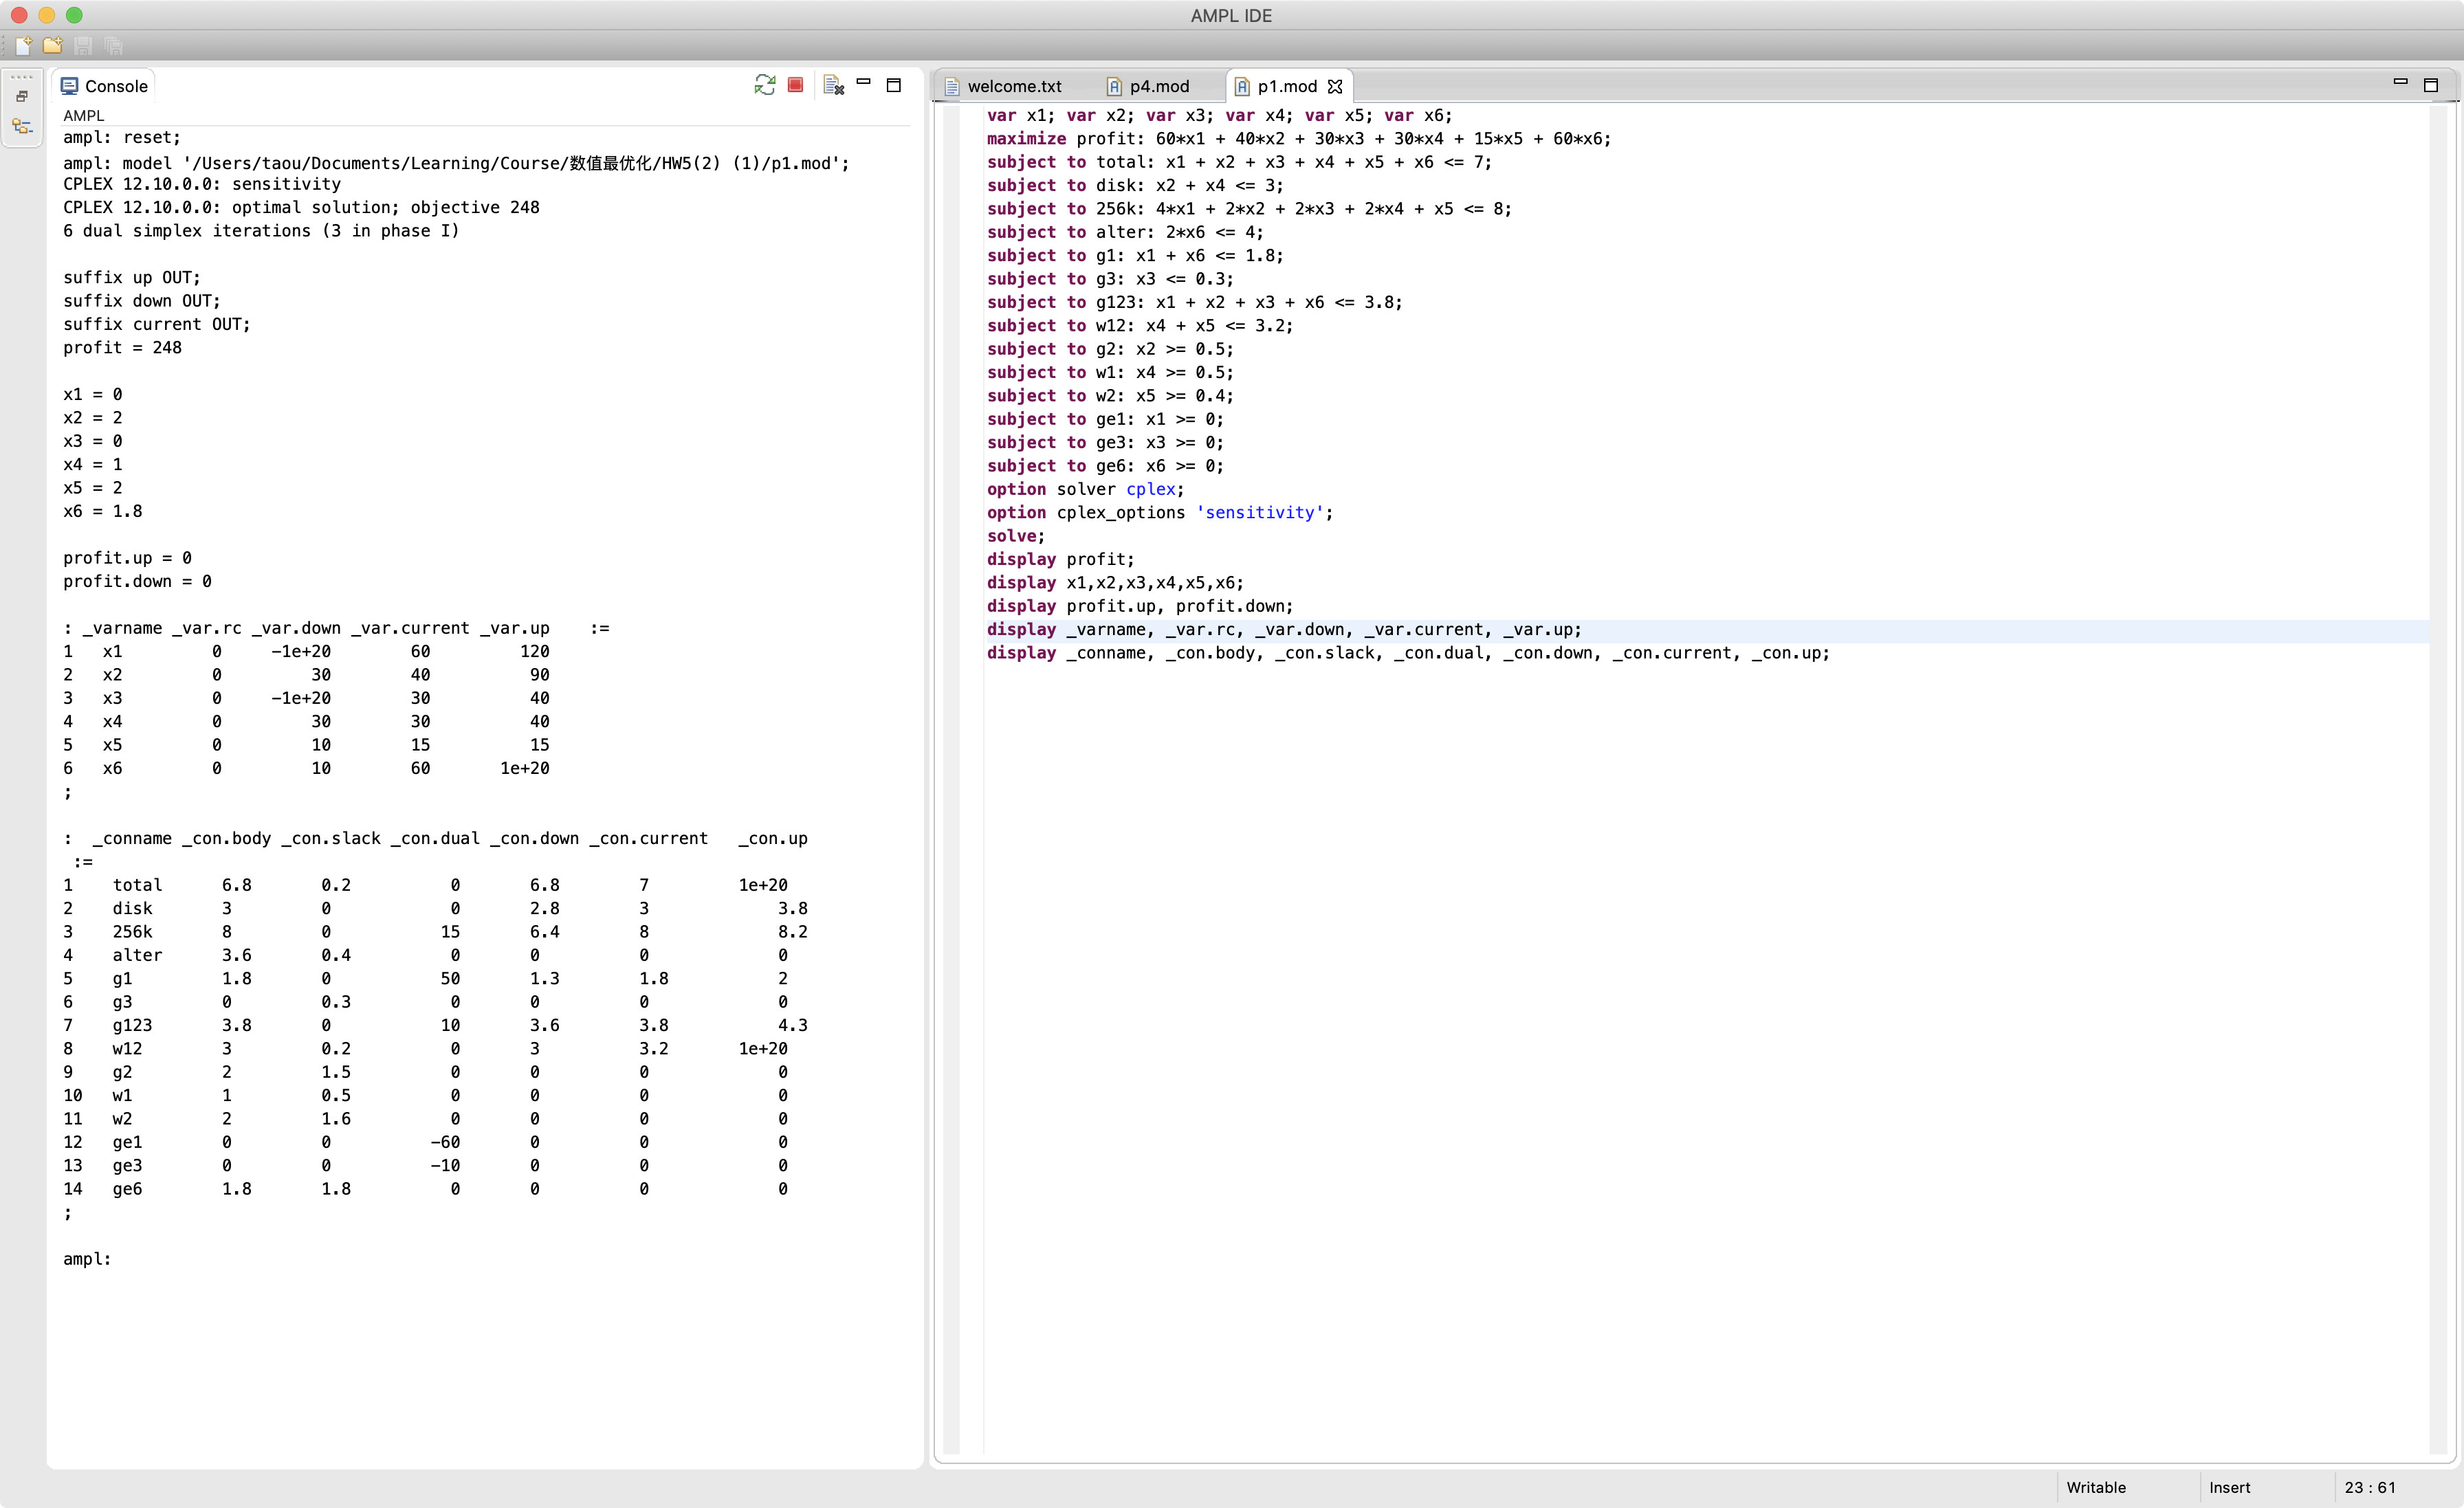
\includegraphics[width=0.8\linewidth]{p1.png}
	%\caption{Accuracy demo.}
	\label{fig.prob2}
	\end{figure}
\end{itemize}


\subsection*{灵敏度分析}
DEC公司为了从四种方案中做出选择, 分别求解了四种方案下对应问题的最优解:
\begin{figure}[H]
	\centering
	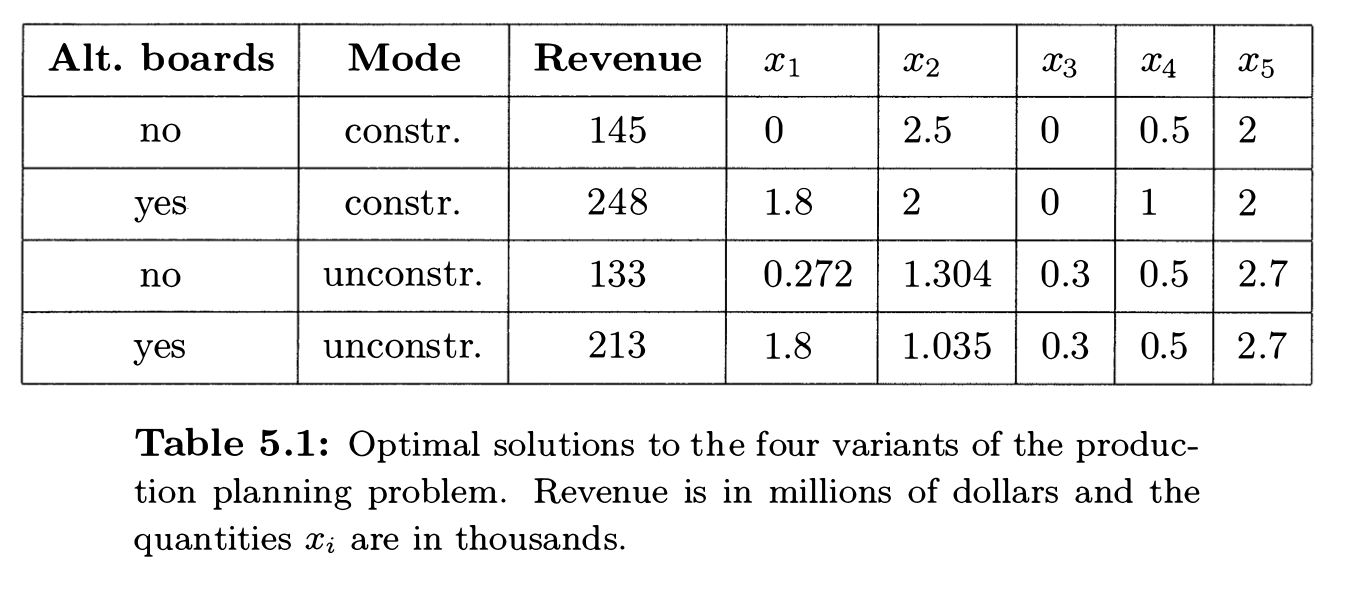
\includegraphics[width=0.7\linewidth]{HW5_2.png}
	%\caption{Accuracy demo.}
	\label{fig.prob2}
\end{figure}
上述表格中易见, alternative mode会带来明显收益, 公司应选择该模式. 而对于是否选择constrained mode则没那么显然. 此外我们上述考虑的线性规划对于disk drives和256K boards的供应量的估计是比较保守的. 因此, 下面我们考虑在问题一解的基础上, 增加disk drives和256K boards的供应量的灵敏度分析问题.

{\color{blue}问题二: 
	\begin{itemize}
		\item[(i)] 用线上的单纯形表法求解器求解问题一中线性规划问题, 附上第一张和最后一张单纯形表的截图. \textcolor{red}{[20pts]}\\
		(可以选择以下网站:\url{https://www.mathstools.com/section/main/simplex_online_calculator}\\
		或 \url{http://simplex.tode.cz/en/} (需要vpn)) 
		\item[(ii)] 根据上一问中的单纯形表, 分析当disk drives和256K boards数量的取值在什么范围内,当前问题的解仍为最优解. 并分析对应的目标函数值将如何变化. \textcolor{red}{[20pts]}
		\item[(iii)] 用AMPL (CPLEX solver)做灵敏度分析检验上一问的结论(disk drives和256K boards数量的取值范围), 给出程序执行结果截图. \textcolor{red}{[20pts]}\\
					( Hint: 查看语句``option cplex\_options `sensitivity';'')
	\end{itemize}
}
\textbf{解}\\
\begin{itemize}
	\item [(i)] 表格如下
	\begin{figure}[H]
	\centering
	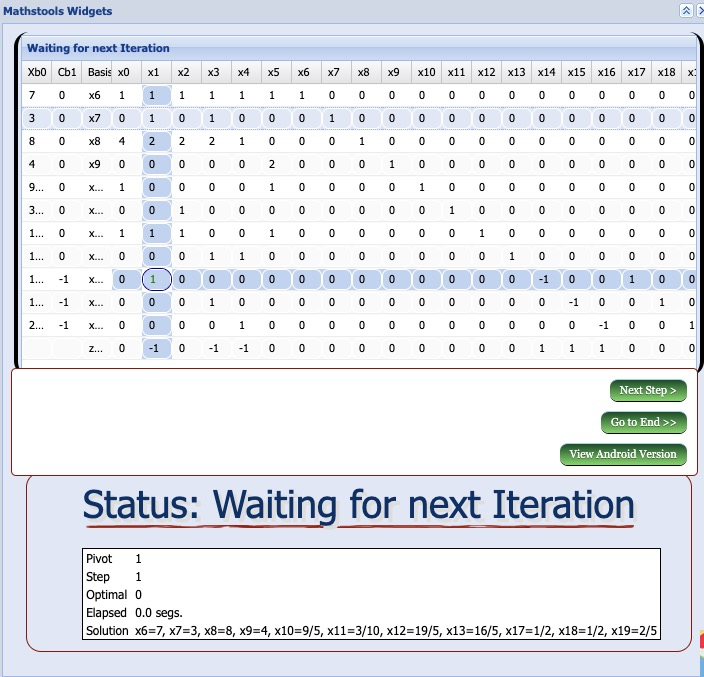
\includegraphics[width=0.7\linewidth]{p2-1.jpg}
	%\caption{Accuracy demo.}
	\label{fig.prob2}
\end{figure}
\begin{figure}[H]
	\centering
	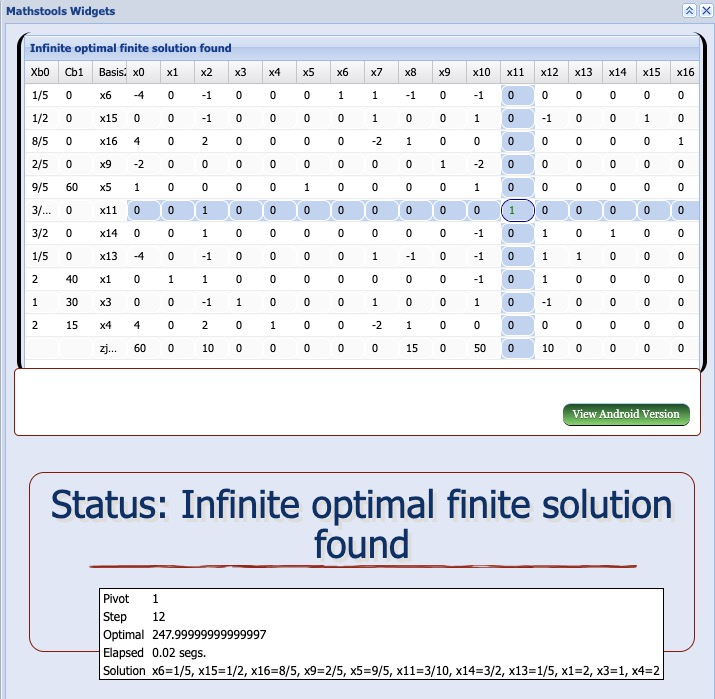
\includegraphics[width=0.7\linewidth]{p2-2.jpg}
	%\caption{Accuracy demo.}
	\label{fig.prob2}
\end{figure}
	\item [(ii)] 根据最后的单纯形表可知,基变量为$x_6,x_{15},x_{16},x_9,x_5,x_{11},x_{14},x_{13},x_1,x_3,x_4$,对应的基矩阵及其逆为
	{\footnotesize
    \begin{align*}B=\left[
\begin{array}{ccccccccccc}
	1 & 0 & 0 & 0 & 1 & 0 & 0 & 0 & 1 & 1 & 1 \\ 
	0 & 0 & 0 & 0 & 0 & 0 & 0 & 0 & 1 & 1 & 0 \\ 
	0 & 0 & 0 & 0 & 0 & 0 & 0 & 0 & 2 & 2 & 1 \\ 
	0 & 0 & 0 & 1 & 2 & 0 & 0 & 0 & 0 & 0 & 0 \\ 
	0 & 0 & 0 & 0 & 1 & 0 & 0 & 0 & 0 & 0 & 0 \\ 
	0 & 0 & 0 & 0 & 0 & 1 & 0 & 0 & 0 & 0 & 0 \\ 
	0 & 0 & 0 & 0 & 1 & 0 & 0 & 0 & 1 & 0 & 0 \\ 
	0 & 0 & 0 & 0 & 0 & 0 & 0 & 1 & 0 & 1 & 1 \\ 
	0 & 0 & 0 & 0 & 0 & 0 & -1 & 0 & 1 & 0 & 0 \\ 
	0 & -1 & 0 & 0 & 0 & 0 & 0 & 0 & 0 & 1 & 0 \\ 
	0 & 0 & -1 & 0 & 0 & 0 & 0 & 0 & 0 & 0 & 1
\end{array}\right]\\
 B^{-1} = \left[
\begin{array}{ccccccccccc}
	1 & 1 & -1 & 0 & -1 & 0 & 0 & 0 & 0 & 0 & 0 \\ 
	0 & 1 & 0 & 0 & 1 & 0 & -1 & 0 & 0 & -1 & 0 \\ 
	0 & -2 & 1 & 0 & 0 & 0 & 0 & 0 & 0 & 0 & -1 \\ 
	0 & 0 & 0 & 1 & 2 & 0 & 0 & 0 & 0 & 0 & 0 \\ 
	0 & 0 & 0 & 0 & 1 & 0 & 0 & 0 & 0 & 0 & 0 \\ 
	0 & 0 & 0 & 0 & 0 & 1 & 0 & 0 & 0 & 0 & 0 \\ 
	0 & 0 & 0 & 0 & -1 & 0 & 1 & 0 & -1 & 0 & 0 \\ 
	0 & 1 & -1 & 0 & -1 & 0 & 1 & 1 & 0 & 0 & 0 \\ 
	0 & 0 & 0 & 0 & -1 & 0 & 1 & 0 & 0 & 0 & 0 \\ 
	0 & 1 & 0 & 0 & 1 & 0 & -1 & 0 & 0 & 0 & 0 \\ 
	0 & -2 & 1 & 0 & 0 & 0 & 0 & 0 & 0 & 0 & 0
\end{array}\right]
\end{align*}}
对于disk drive和256k board, 对应着$B^{-1}$的第二列和第三列,根据可行性条件
$$B^{-1}(b+\delta)\ge 0$$
可得
$$x_{B(2)}+\delta \beta_{2i}\ge 0$$
$$x_{B(2)}+\delta \beta_{3i}\ge 0$$
等价于
$$\max_{\beta{2i}>0}(-\frac{x_{B(2)}}{\beta_{2i}})\le \delta\le \min_{\beta_{2i}>0}(-\frac{x_{B(2)}}{\beta_{2i}})$$
$$\max_{\beta{3i}>0}(-\frac{x_{B(3)}}{\beta_{3i}})\le \delta\le \min_{\beta_{3i}>0}(-\frac{x_{B(3)}}{\beta_{3i}})$$
由此可得
$$-0.2\le\delta_{disk}\le0.8,-1.6\le\delta_{256k}\le 0.2\quad(\text{对应}\beta_{2i},\beta_{3i})$$
即disk的取值在(2.8,3.8)之间,256k board取值在(6.4,8.2)之间。\\
对于目标函数的变化,由公式$c_B^TB^{-1}e_{i}$可得
$$\text{disk: } c_B^TB^{-1}e_{2} = (0,0,0,0,60,0,0,0,40,30,15)\cdot (1,1,-2,0,0,0,0,1,0,1,-2) = 0$$
$$\text{256k board: } c_B^TB^{-1}e_{3} = (0,0,0,0,60,0,0,0,40,30,15)\cdot (-1,0,1,0,0,0,0,-1,0,0,1) = 15$$
即改变单位(1k)的disk不会影响收益,改变单位(1k)的256k board会增加15k的收益。
\item [(iii)] 由灵敏度分析结果可知(line2,3),disk的取值在(2.8,3.8)之间,256k board取值在(6.4,8.2)之间,验证了第二问中的结论。
\begin{figure}[H]
	\centering
	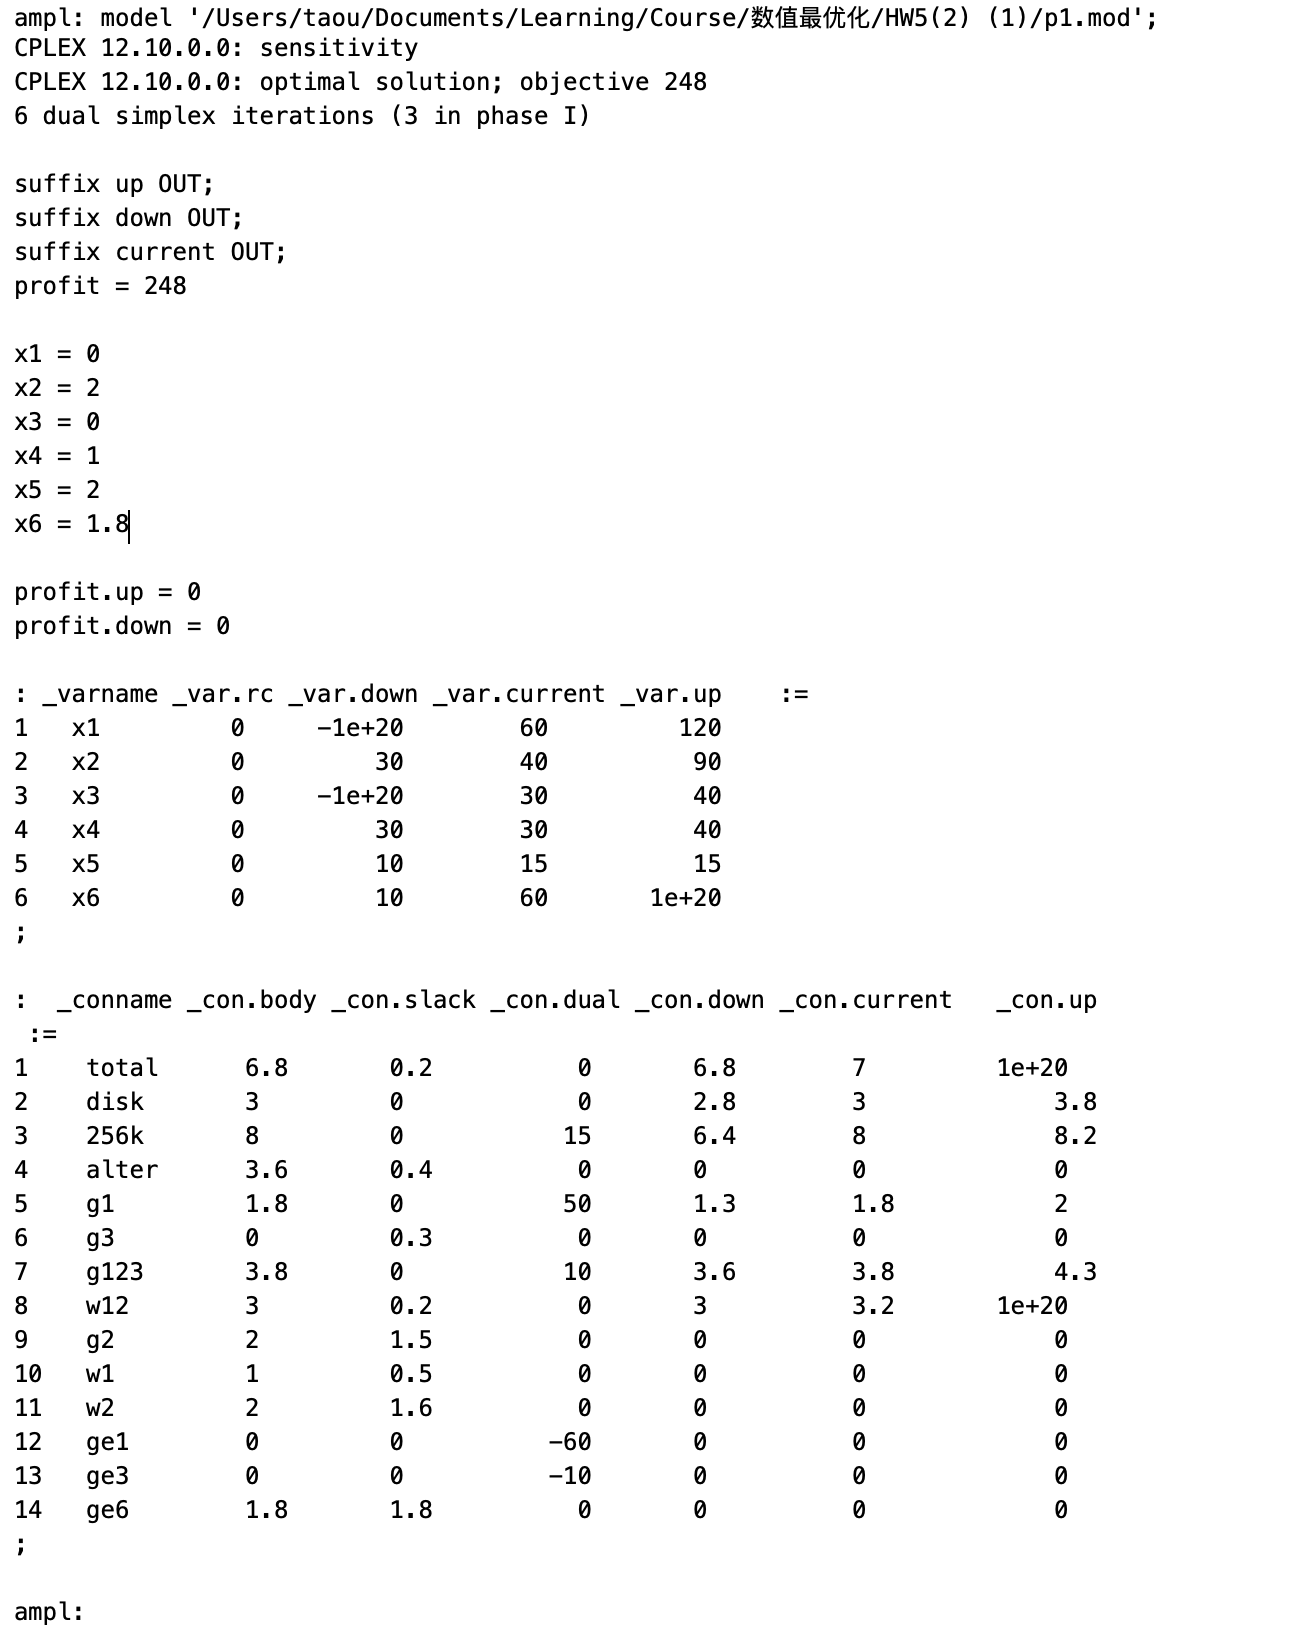
\includegraphics[width=0.5\linewidth]{p2-3.png}
	%\caption{Accuracy demo.}
	\label{fig.prob2}
\end{figure}
\end{itemize}
\end{document} 